\documentclass[11pt]{article}
\usepackage{amsmath,amssymb,color,float}
\usepackage{stmaryrd}
\usepackage{graphicx,psfrag,epsf}
\usepackage[authoryear]{natbib}
\usepackage{fullpage,setspace}
\usepackage{subcaption}
\usepackage{changepage}
\usepackage{listings}
\usepackage{comment}

\setlength{\oddsidemargin}{.15in} 
\setlength{\textwidth}{6.25in}
\setlength{\topmargin}{-0.25in}
\setlength{\headheight}{-0.15in}
\setlength{\textheight}{8.9in} 

\linespread{1.25}

\title{ST793 Project: A Blogpost on ``Doubly Enhanced EM Algorithm for Model-Based Tensor Clustering" by Mai et al}
\author{Ayumi Mutoh, Jisu Oh, Shih-Ni Prim}

\begin{document}

\maketitle

\section{Introduction}

In recent decades, tensor data have gained popularity in modern science, their high-dimensional structures often pose challenges for statistical analysis, specifically in model-based clustering. Model-based clustering is a statistical approach to data clustering, where observed data is considered to have been created from a finite combination of component models, such as the Gaussian mixture model (GMM). Since the formalization of the expected-maximization (EM) algorithm by \cite{dempster1977EM}, the EM algorithm has been widely employed in the majority of model-based clustering applications. While the GMMs can be readily extended to higher-order tensors using the standard EM algorithm, their performance can be further enhanced by integrating the DEEM algorithm, as proposed by \cite{mai2022DEEM}. Mai et al. consider a tensor normal mixture model (TNMM) that incorporates tensor correlation structure and variable selection for clustering and parameter estimation. They developed the DEEM algorithm which enables DEEM to excel in high-dimensional tensor data analysis. Similar to the EM algorithm, DEEM carries out an enhanced E-step and an enhanced M-step. 

In this blogpost, we first introduce the DEEM methods with intermediate
steps for the theoretical explanation. The objective is to break down the steps, making the derivation more accessible for our readers to follow. Subsequently, we will conduct a simulation study to evaluate the performance of DEEM.

 
\section{Theoretical Derivation}
\subsection{EM Algorithm}
Before delving into DEEM, we would like to review the EM algorithm and its functioning in clustering.

As we have learned in class, the EM algorithm is an iterative approach that cycles between two steps for maximum likelihood estimation in the presence of latent variables. The observed data Y is incomplete and data Z is missing. The first step is to write down the joint likelihood, $L_c(
\theta|Y,Z)$, of the ``complete" data $(Y,Z)$. The ``E" step of the EM algorithm is to compute the conditional expectation of log-likelihood, $\text{log}L_c(
\theta|Y,Z)$, given Y assuming the true parameter value is $\theta^{(\nu)}$
\[Q(\theta,\theta^{(\nu)},Y)=E_{\theta^{(\nu)}}(\text{log}L_c(
\theta|Y,Z)|Y).\] In the ``M" step, we maximize $Q(\theta,\theta^{(\nu)},Y)$ with respect to $\theta$ with $\theta^{(\nu)}$ fixed. 
\begin{comment}
    \begin{itemize}
    \item \textbf{E-step}: Estimate the missing or latent variables  
    \item \textbf{M-step}: Maximize the parameters of the model 
\end{itemize}
\end{comment}

The EM algorithm is well-known for use in unsupervised learning problems such as clustering with a mixture model. The process goes as follows:
\begin{enumerate}
    \item Identify the number of clusters. 
    \item Define each cluster by generating a Gaussian model. 
    \item For every observation, calculate the probability that it belongs to each cluster (Ex. observation 12 has 40\% probability of belonging to Cluster A and 60\% probability of belonging to Cluster B.)
    \item Using the above probabilities, recalculate the Gaussian models. 
    \item Repeat until observations ``converge" on their assignments. 
\end{enumerate}

Let's consider a simple example. Suppose we have data $X_i$ as shown in Figure \ref{fig:clustering1}, which comes from two distinct classes. We use this data to build a Gaussian model for each class. Since we don't know which class each observation belongs to, there is no straightforward way to construct two Gaussian models to partition the data. Therefore, we begin with a random guess of our Gaussian model parameters: $\mu_1,\sigma^2_1, \mu_2,\sigma^2_2$. 

We have `missing' data points $X_i$ that we believe belong to either of the two distributions. After initializing two random Gaussian models, we compute the likelihood of each observation, $X_i$, being expressed in both of the Gaussian models. The next is the E-step, where we compute the probability that each $X_i$ can belong to any of two distributions. Now we have a probability of belonging to either distribution for each point. 

In the M-step, we update the parameters, $\mu_1,\sigma^2_1, \mu_2,\sigma^2_2$, of the model to their most likely values. For the new $\mu_1$, we take a weighted average of all the points, weighted by the probability that they belong to the first distribution. Denoting $p_i$ is the probability that $X_i$ belongs to the first distribution. 
\[\mu_1=\frac{p_1X_1+p_2X_2+\dots+p_nX_n}{p_1+p_2+\dots+p_n}\]
The new $\sigma^2_1$ can be updated similarly. 
\[\sigma^2_1=\frac{p_1(X_1-\mu_1)^2+p_2(X_2-\mu_1)^2+\dots+p_n(X_n-\mu_1)^2}{p_1+p_2+\dots+p_n}\]
We repeat this process for $\mu_2$ and $\sigma^2_2$ and update our distributions. We iterate through the E-step and M-step until convergence, obtaining two clusters as shown in Figure \ref{fig:clustering2}. 




\begin{figure}
    \centering
    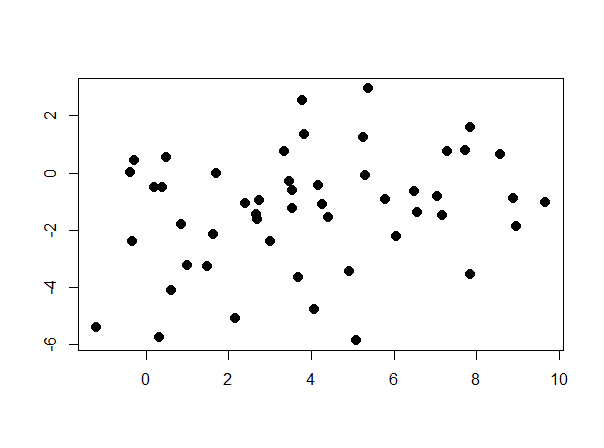
\includegraphics[width = 10 cm]{nocolor.png}
    \caption{Mixture of two Gaussian Distributions}
    \label{fig:clustering1}
\end{figure}


\begin{figure}
    \centering
    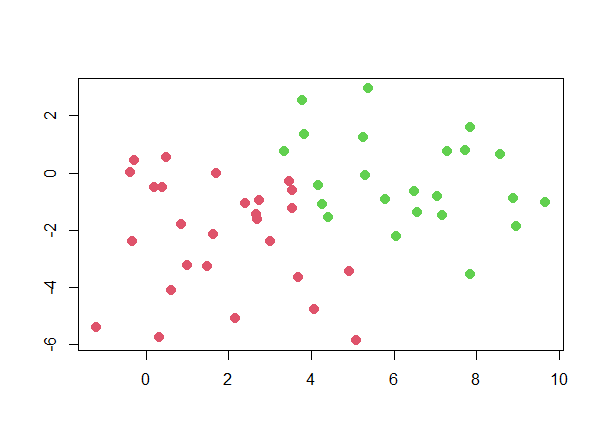
\includegraphics[width = 10 cm]{clustering.png}
    \caption{Clusters Found by EM algorithm}
    \label{fig:clustering2}
\end{figure}


\subsection{Tensor}

While the term ``tensor" might sound unfamiliar to some, tensors are simply multi-way arrays. Data is often structured as matrices, and they are in fact second-order tensors. When we use the term ``tensor," we usually mean tensors of third-order and higher. You can think of a third-order tensor as a cube. There are then three dimensions from which to look at the tensor. These three dimensions are called ``modes."  If you are interested in knowing more about tensors, a very popular and highly cited paper by \cite{kolda2009review} has lots of great details. So check it out! A figure from this paper is included in our Figure \ref{fig:tensor} to give you an idea of the different ways to look at a tensor. For this blogpost, we will focus on the method DEEM by \cite{mai2022DEEM}, so we will not delve into more details about tensors and will focus on how this method is an upgrade of the classical EM algorithm.

\begin{figure}
    \centering
    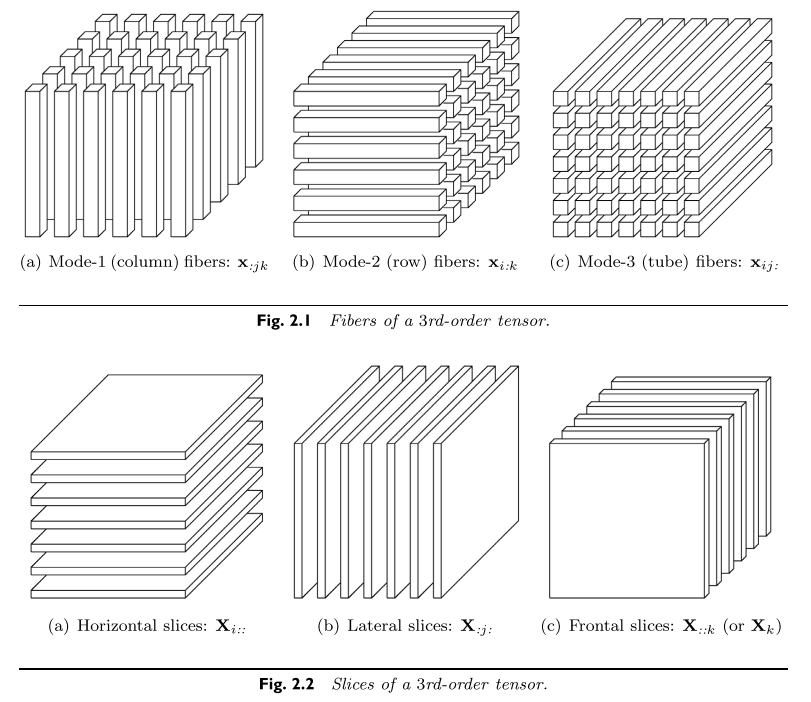
\includegraphics[width = 10 cm]{tensor.png}
    \caption{Dimensions and Terminology of a Tensor (from \cite{kolda2009review})}
    \label{fig:tensor}
\end{figure}

\subsection{Doubly Enhanced EM Algorithm}

\section{Simulation Study}

\subsection{Data Generation}

For our simulation studies, we follow the framework used in \cite{mai2022DEEM}. For each setting, $K$ denotes the number of mixture groups, and noise is generated as a $M^{th}$-order tensor:  
\begin{equation}
    \mathbf{X}_i \sim \sum_{k=1}^K \pi^*_k \mbox{TN} (\boldsymbol{\pi}^*_k; \boldsymbol{\Sigma}^*_1, \cdots, \boldsymbol{\Sigma^*_M}), i = 1, \cdots, n
\end{equation}
For $K-1$ mixture groups, the $\mathbf{X}_i$ is given as a given $\mathbf{B}_k$ plus the noise above. For $1$ mixture group, the values are simply the noise. \cite{mai2022DEEM} designate two types of $\boldsymbol{\Sigma}^*_k$: 
\[  \boldsymbol{\Omega} =   \begin{cases}
     AR(\rho): & \omega_{ij} = \rho^{|i-j|} \\
    CS(\rho): & \omega_{ij} = \rho + (1-\rho) 1(i=j).
\end{cases}\]
For each setting, we generate $100$ independent datasets, the same number of replicates as \cite{mai2022DEEM} use, and present the mean error rate and standard deviation. 

\subsection{Settings}

The settings are provided in Table \ref{tab:sim_setting}. Note that, for ${B}^*_{k}$, the indices not included in the subscript is $0$. In other words, ${B}^*_k$ is a sparse tensor. We chose these four settings from the seven settings, because their settings are increasingly more computationally expensive, and we believe that these four settings demonstrate the advantage of the DEEM algorithm compared to the classical EM algorithm in terms of accuracy, as shown in Table \ref{tab:err}. 

\begin{table}[ht]
    \centering
    \begin{tabular}{c|p{4in}}
      Model & Parameters \\
    \hline
    M1  & $K=2, p = 10\times 10 \times 4, \boldsymbol{\Sigma}^*_1 = CS(0.3), \boldsymbol{\Sigma}^*_2 = AR(0.8), \boldsymbol{\Sigma}^*_3 = CS(0.3), \mathbf{B}^*_{2,[1:6,1,1]} = 0.5$  \\
    \hline
    M3 &  $K=3, p = 10\times 10 \times 4, \boldsymbol{\Sigma}^*_1 = CS(0.3), \boldsymbol{\Sigma}^*_2 = AR(0.8), \boldsymbol{\Sigma}^*_3 = CS(0.5), \mathbf{B}^*_{2,[1:6,1,1]} = 0.5, \mathbf{B}^*_{3,[1:6,1,1]} = -0.5$  \\
    \hline
    M4 &  $K=4, p = 10\times 10 \times 4, \boldsymbol{\Sigma}^*_1 = \mathbf{I}_{10}, \boldsymbol{\Sigma}^*_2 = AR(0.8), \boldsymbol{\Sigma}^*_3 = \mathbf{I}_4, \mathbf{B}^*_{2,[1:6,1,1]} = 0.8, \mathbf{B}^*_{3,[1:6,1,1]} = -0.8$ \\
    \hline
    M5 &  $K=6, p = 10\times 10 \times 4, \boldsymbol{\Sigma}^*_1 = AR(0.9), \boldsymbol{\Sigma}^*_2 = CS(0.6), \boldsymbol{\Sigma}^*_3 = AR(0.9), \mathbf{B}^*_{2,[1:6,1,1]} = 0.6, \mathbf{B}^*_{3,[1:6,1,1]} = 1.2, \mathbf{B}^*_{4,[1:6,1,1]} = 1.8, \mathbf{B}^*_{5,[1:6,1,1]} = 2.4, \mathbf{B}^*_{6,[1:6,1,1]} = 3$ 
    \end{tabular}
    \caption{Simulation settings}
    \label{tab:sim_setting}
\end{table}

\subsection{Metrics}

Note that it is as straightforward to calculate the mean error rate for a clustering problem than it is for a classification problem. Both methods return labels for the groups; however, the group labels do not matter. For example, if there are five observations and if their true group labels are $(1,1,2,2,2)$ and the methods return $(2,2,1,1,1)$, the error rate should be $0$. In the paper, the authors explain that mean clustering error rate is calculated by: 
\[ \min_\prod \frac{1}{n} \sum_{i=1}^n 1 (\hat{Y}_i \ne \prod (Y_i)) \text{ over all possible permutations } \prod: \{1, \cdots,  \} \mapsto \{1, \cdots, K\} \]
We thus created a function to permute the true labels, compare the estimated labels and the true labels, and return the lowest error rate. 

To compare the speed of the two methods, we also record the computation time. Table \ref{tab:time} provides the mean computation time and standard error (in parentheses) for each setting. 

\subsection{External R Packages and Functions}

For the DEEM algorithm, we use the function DEEM; for the standard EM algorithm, we use the function TGMM. Both functions are from the R package TensorClustering. We use the Trnorm function from the R package Tlasso to generate tensor noise with designated covariance matrices. We use the permutations function in the gtools package to permute true labels. In short, be sure to install the three R packages: TensorClustering, Tlasso, and gtools if you would like to reproduce our simulation. 


\subsection{Simulation result}

The error rates and computation time are shown in Tables \ref{tab:err} and \ref{tab:time}. It is clear that DEEM has lower mean error rates in all four settings. The computation time tells a different story, however. As seen in Table \ref{tab:time}, DEEM is not always the winner in terms of time. As the setting becomes more complicated and estimating the clusters becomes more challenging, it takes longer for DEEM to converge. In fact, judging from the amount of time it took to run the setting M5, it is possible that DEEM reached the maximum iterations. 

\begin{table}[ht]
    \centering
    \begin{tabular}{c|cc}
       Model  &  DEEM & EM \\
       \hline
         M1 & 0.41 (0.05) & 0.45 (0.03) \\
         M3 &  0.46 (0.09) & 0.56 (0.05) \\
         M4 &  0.35 (0.03) & 0.57 (0.06) \\ 
         M5 &  0.31 (0.11) & 0.43 (0.06) \\
    \end{tabular}
    \caption{Error Rates from 100 Replicates}
    \label{tab:err}
\end{table}

\begin{table}[ht]
    \centering
    \begin{tabular}{c|cc}
       Model  &  DEEM & EM \\
       \hline
         M1 & 0.72 (0.45) & 0.93 (0.39) \\
         M3 &  13.95 (7.78) & 7.74 (3.99) \\
         M4 &  15.8 (0.81) & 21.9 (9.68) \\ 
         M5 &  332.96 (124.38) & 14.66 (5.88) \\
    \end{tabular}
    \caption{Computation Time (seconds) from 100 Replicates}
    \label{tab:time}
\end{table}

Next we transform the values in the tables into figures, which sometimes tell clearer pictures. As shown in Figure \ref{fig:err}, DEEM always has lower mean error rates. However, as the model becomes complicated, DEEM's error rates become more varied, even though the mean rate is still lower. In Figure \ref{fig:time}, the story seems more complicated. (Note that we cannot make the y-axis all the same for the four plots, because the computation time for DEEM for M5 is so long, which would make some of the boxes very small and not informative.) For the two settings M1 and M4, DEEM has lower computation time. For M3, the computation time for DEEM is much more varied, and EM has overall shorter computation time. For M5, DEEM has very long computation time; in fact, the 100 replicates took almost 10 hours to run. It is unclear if the reduction in error rate is worht the much longer computation time.

\begin{figure}
    \centering
    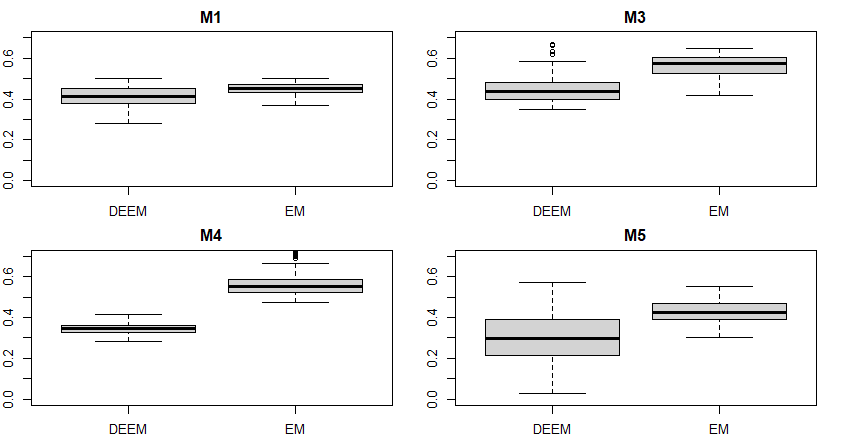
\includegraphics[width = 16 cm]{sim_error.png}
    \caption{Boxplots of Mean Error Rates from 100 Replicates}
    \label{fig:err}
\end{figure}

\begin{figure}
    \centering
    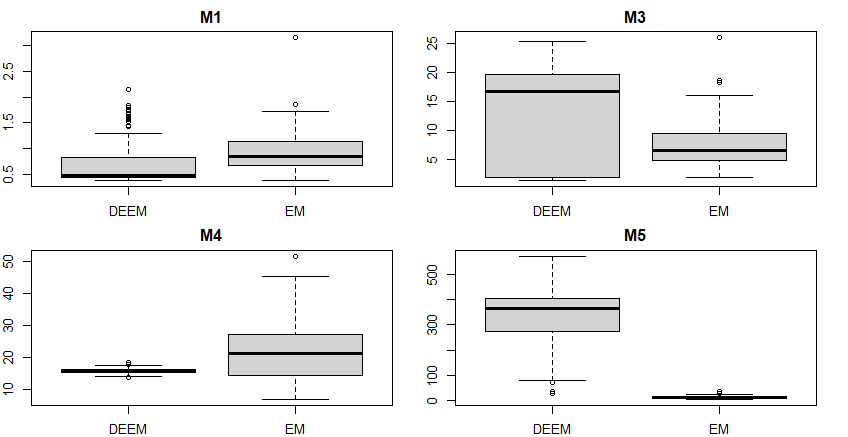
\includegraphics[width = 16 cm]{sim_time.png}
    \caption{Boxplots of Mean Computation Time (in seconds) from 100 Replicates}
    \label{fig:time}
\end{figure}




\section{Discussion}

In this blogpost, we review a new method proposed by \cite{mai2022DEEM}, which is essentially an upgraded version of the classical EM algorithm. This new method, DEEM, tend to have lower error rates on tensor data. However, the running time could be prohibitive. 

\section{Conclusion}

[to be added]

\begin{singlespace}
	\bibliographystyle{rss}
	\bibliography{refs}
\end{singlespace}


\end{document}